%%%%%%%%%%%%%%%%%%%%%%%%%%%%%%%%%%%%%%%%%%%%%%%%%%%%%%%%%%%%%%%%%%%%%%%%
\chapter{Introduction}
\label{chapter:ch1-introduction}
%%%%%%%%%%%%%%%%%%%%%%%%%%%%%%%%%%%%%%%%%%%%%%%%%%%%%%%%%%%%%%%%%%%%%%%%
\localtoc

%%%%%%%%%%%%%%%%%%%%%%%%%%%%%%%%%%%%%%%%%%%%%%%%%%%%%%%%%%%%%%%%%%%%%%%%%%%%%%%
\section{Context and Motivation}
\label{section:ch1-context_and_motivation}
%%%%%%%%%%%%%%%%%%%%%%%%%%%%%%%%%%%%%%%%%%%%%%%%%%%%%%%%%%%%%%%%%%%%%%%%%%%%%%%


\begin{figure}[t]
  \centering
  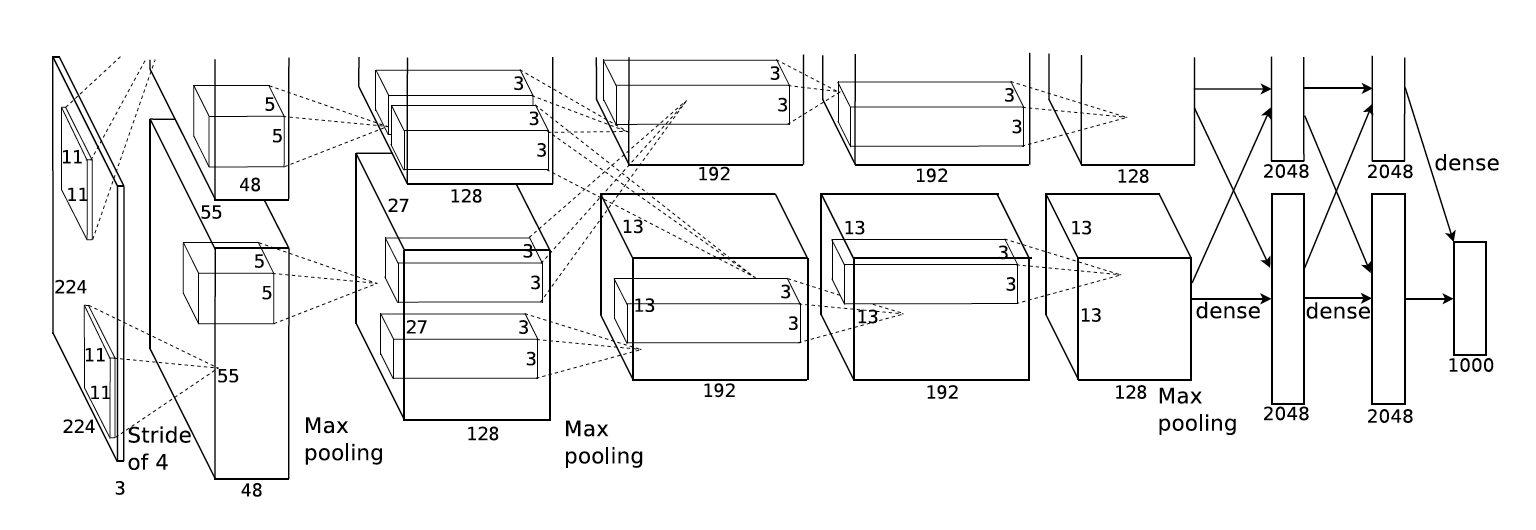
\includegraphics[scale=0.22]{figures/main/ch1-introduction/alexnet.png}
  \caption{The neural network architecture (AlexNet) proposed by~\citet{krizhevsky2012imagenet} which won the ImageNet Large-Scale Visual Recognition Challenge in 2012.}
  \label{figure:ch1-alexnet_network}
\end{figure}


One of the most remarkable breakthroughs of Deep Learning happened during the 2012 ImageNet Large-Scale Visual Recognition Challenge~\cite{ILSVRC15} which consists of evaluating algorithms for object detection and image classification.
During this challenge, \citet{krizhevsky2012imagenet} achieved \nth{1} place and beat every other participant by a 10.8\% margin with a neural network architecture called \textbf{AlexNet}.
The main reasons for this success are twofold.
First of all, they used a convolutional neural network (CNN) with more than 60 million parameters which was one of the largest models of the time.
% Secondly, with 1.2 million labeled images, the ImageNet database~\cite{deng2009imagenet} was an adequate dataset to train a neural network with so many parameters.
Secondly, they designed a specific architecture to exploit dual programmable graphics processing units (GPUs) to speed up the arithmetic operations, which enabled them to significantly reduce training time.
% Finally, they used programmable graphics processing units (GPUs) to speed up the arithmetic operations, which enabled them to significantly reduce training time.
The \Cref{figure:ch1-alexnet_network} shows the AlexNet architecture which consists of five convolutional layers with two fully connected layers at the end.
The figure also shows the distribution of the workload between the two GPUs.

% 1 ils ont concu un model enorme
% 2 ils ont concu une archiecture pour entrainer ce model enorme


\begin{table}[t]
  \centering
  \sisetup{
    table-number-alignment = center,
    table-space-text-pre = \ \ \ ,
  }
  \begin{subfigure}[b]{\textwidth}
    \centering
    \begin{tabular}{
      L{5cm}
      L{3.5cm}
      S[table-format=3.0, table-text-alignment=left]@{\,}
      s[table-unit-alignment=left]
      c
    }
      \toprule
      \textbf{Authors} & \textbf{Models} & \multicolumn{2}{c}{\textbf{\#Params}} & \textbf{TOP-5 Acc.} \\
      \midrule
      \citet{krizhevsky2012imagenet} & AlexNet             &  61 & \si{M} & 84.7\% \\
      \citet{simonyan2014very}       & VGG                 & 144 & \si{M} & 92.0\% \\
      \citet{he2016deep}             & ResNet-152          &  60 & \si{M} & 93.8\% \\
      \citet{szegedy2017inception}   & Inception-ResNet-v2 &  56 & \si{M} & 95.1\% \\
      \citet{xie2017aggregated}      & ResNeXt-101         &  84 & \si{M} & 95.6\% \\
      \citet{hu2018squeeze}          & SENet               & 146 & \si{M} & 96.2\% \\
      \citet{real2019regularized}    & AmoebaNet-A         & 469 & \si{M} & 96.7\% \\
      \citet{huang2019gpipe}         & AmoebaNet-B         & 556 & \si{M} & 97.0\% \\
      \bottomrule
    \end{tabular}
    \caption{Computer Vision Models}
    \label{table:ch1-networks_parameters_cv}
  \end{subfigure}
  \par\bigskip
  \begin{subfigure}[b]{\textwidth}
    \centering
    \begin{tabular}{
      L{4.5cm}
      L{4.5cm}
      S[table-format=3.0, table-text-alignment=left]@{\,}
      s[table-unit-alignment=left]
    }
      \toprule
      \textbf{Authors} & \textbf{Models} & \multicolumn{2}{c}{\textbf{\#Params}} \\
      \midrule
      \citet{peters2018deep}         & ELMo            &  94 & \si{M} \\
      \citet{radford2018improving}   & GPT             & 110 & \si{M} \\
      \citet{devlin2019bert}         & BERT            & 340 & \si{M} \\
      \citet{yang2019xlnet}          & XLNet (Large)   & 340 & \si{M} \\
      \citet{liu2019roberta}         & RoBERTa (Large) & 355 & \si{M} \\
      \citet{radford2019language}    & GPT-2           &   1 & \si{B} \\
      \citet{shoeybi2019megatron}    & MegatronLM      &   8 & \si{B} \\
      \citet{raffel2020exploring}    & T5-11B          &  11 & \si{B} \\
      \citet{rosset2020turingnlg}    & T-NLG           &  17 & \si{B} \\
      \citet{brown2020language}      & GPT-3           & 175 & \si{B} \\
      \citet{fedus2021switch}        & Switch Transformers & 1 & \si{T} \\
      \bottomrule
    \end{tabular}
    \caption{Natural Language Processing Models}
    \label{table:ch1-networks_parameters_nlp}
  \end{subfigure}
  \caption{
    Tables showing the different network architectures developed in the years after AlexNet.
    \Cref{table:ch1-networks_parameters_cv} shows networks developed for computer vision tasks and \Cref{table:ch1-networks_parameters_nlp} shows networks developed for natural language processing.
  }
  \label{table:ch1-networks_parameters}
\end{table}


Following this result, many architectures with an increasing number of parameters have been developed.
This growth in the number of parameters has led to an increase in accuracy exceeding human performance on the ImageNet dataset~\cite{he2015delving}.
\Cref{table:ch1-networks_parameters} shows an historic of the different state-of-the-art architectures along with their size, and accuracy.
As we can see, the accuracy of the models generally improves at the cost of the model size.
% This increase in model size has been possible with the increase in computational resources~\cite{huang2019gpipe} and the availability of high level deep learning frameworks~\cite{tensorflow2015-whitepaper,paszke2019pytorch}.
% While most new architectures have been proposed based on empirical studies, recent research \cite{tan2019efficientnet,rosenfeld2020a} have examined the relationship between the number of parameters (model size), the size of the dataset and the accuracy.
For computer vision models, \citet{tan2019efficientnet} have shown that the relationship between model size and accuracy seems to obey a power law.
% This discovery led them to develop a new scaling method that balances all dimensions of network width, depth, and resolution, leading to an efficient neural network with similar or higher accuracy than current ones.
This relationship has also been observed for Natural Language Processing (NLP) neural networks \cite{rosenfeld2020a,kaplan2020scaling} and given the availability of large-scale datasets (Common Crawl dataset~\cite{raffel2019exploring} constitutes nearly a trillion words), researchers have been able to scale their models.
GPT-3 model, one of the latest models proposed by~\citet{brown2020language}, culminates at 175 billion parameters and requires 355 years of training on a single GPU and \$4,600,000 to train on a cloud computing platform \cite{li2020overview}.
Furthermore, \citet{strubell2019energy} estimated model training and development costs in terms of $\mathrm{CO}_2$ emissions.
For example, training the large Transformer model proposed by~\cite{vaswani2017attention} with neural architecture search emits an estimated \numprint{284019} kg of $\mathrm{CO}_2$ whereas a human life will consume an average of \numprint{5000} kg of $\mathrm{CO}_2$ for one year.

As a result of their size and improved accuracy, deep neural networks now achieve state-of-the-art performances in a variety of domains such as image recognition~\cite{lecun1998gradient,krizhevsky2012imagenet,he2016deep,tan2019efficientnet}, object detection~\cite{redmon2016you,liu2016ssd,redmon2017yolo9000}, natural language processing~\cite{merity2016pointer,vaswani2017attention,radford2018Language,brown2020language}, speech recognition~\cite{hinton2012deep,abdel2014convolutional,yu2016automatic}, health care \cite{faust2018deep} etc.
Specifically, computer vision and natural language processing models have achieved sufficient performance for being used in real-world applications such as autonomous vehicles~\cite{fagnant2015preparing,sharma2021automating}, translation~\cite{wu2016google}, vocal assistants~\cite{li2017acoustic}, etc.

% However, recent findings suggest that the accuracy cannot be the only metric to optimize.
However, accuracy is not the only concern, when implemented in a critical decision process, neural networks need to be compact, cost effective and secure.
Although accurate, large neural networks often lack these properties.
Indeed, large neural networks require a large amount of computing power limiting their access to many small research labs and companies.
Furthermore, large and deep neural networks have shown to be unreliable in certain circumstances, \ie, they have been shown to be vulnerable to adversarial examples, raising many societal problems (judicial decision, self-driving cars, etc.).
This thesis focuses on the problem of training neural networks which are not only accurate, but also compact, easy to train, reliable and robust to adversarial examples.

% In recent years, deep neural networks have grew larger and larger both in terms of depth and number of parameters.
% Although accurate, large neural networks  exhibit important drawbacks.
%
% The existence of adversarial examples poses a growing societal problem as more and more machine learning models are trained and deployed in critical decision system.
% Indeed, they call into question the reliability of neural networks, and their use in a context where the presence of malicious users is to be expected.
% My research goals aim at solving this important problem.

%%%%%%%%%%%%%%%%%%%%%%%%%%%%%%%%%%%%%%%%%%%%%%%%%%%%%%%%%%%%%%%%%%%%%%%%%%%%%%%
\section{Problem Statement}
\label{section:ch1-problem_setting}
%%%%%%%%%%%%%%%%%%%%%%%%%%%%%%%%%%%%%%%%%%%%%%%%%%%%%%%%%%%%%%%%%%%%%%%%%%%%%%%


\begin{figure}[t]
   \centering
   \begin{subfigure}[t]{0.24\textwidth}
       \centering
       \begin{equation*}
	  \leftmatrix
	    a &   &   &   \\
	      & b &   &   \\
	      &   & c &   \\
	      &   &   & d
	  \rightmatrix
       \end{equation*}
       \caption*{diagonal}
   \end{subfigure}
   \hfill
   \begin{subfigure}[t]{0.24\textwidth}
       \centering
       \begin{equation*}
	  \leftmatrix
	    a & b & c & d \\
	    e & a & b & c \\
	    f & e & a & b \\
	    d & f & e & a
	  \rightmatrix
       \end{equation*}
       \caption*{Toeplitz}
   \end{subfigure}
   \hfill
   \begin{subfigure}[t]{0.24\textwidth}
       \centering
       \begin{equation*}
	  \leftmatrix
	    ae & af & ag & ah \\
	    be & bf & bg & bh \\
	    ce & cf & cg & ch \\
	    de & df & dg & dh
	  \rightmatrix
       \end{equation*}
       \caption*{Low Rank}
   \end{subfigure}
   \hfill
   \begin{subfigure}[t]{0.24\textwidth}
       \centering
       \begin{equation*}
	  \leftmatrix
	    a & a^2 & a^3 & a^4 \\
	    b & b^2 & b^3 & b^4 \\
	    c & c^2 & c^3 & c^4 \\
	    d & d^2 & d^3 & d^4
	  \rightmatrix
       \end{equation*}
       \caption*{Vandermonde}
   \end{subfigure}
  \caption{Examples of structured matrices.}
  \label{figure:ch1-example_structure_matrices}
\end{figure}


% In this thesis, we focus on the design and the training of \emph{neural networks} that are cost-effective, compact and secure.

Neural networks, which find their roots in the work of \citet{mcculloch1943logical,rosenblatt1958perceptron}, can be analytically described as a composition of multi-dimensional linear functions interlaced with nonlinear functions (also called activation functions).
More precisely, a neural network is a function $N_{\Omega} : \Rbb^n \rightarrow \Rbb^m$ parameterized by $\Omega$ which can be expressed as follows:
\begin{equation} \label{equation:ch1-neural_network}
  N_{\Omega}(\xvec) = \psi^{(\depth)} \circ \rho \circ \psi^{(\depth-1)} \cdots \circ \psi^{(2)} \circ \rho \circ \psi^{(1)} (\xvec)
\end{equation}
where $\depth$ corresponds to the \emph{depth} of the network (\ie, the number of layers), $\rho$ is a nonlinear function and $\psi^{(i)}$ are multi-dimensional linear functions of the form $\xvec \mapsto \Wmat^{(i)} \xvec + \bvec^{(i)}$ where $\Wmat^{(i)}$ is a matrix called the \emph{weight} matrix of the layer $i$ and $\bvec^{(i)}$ is the bias (we present a more formal definition of neural networks in~\Cref{chapter:ch2-background}).

% Neural networks can be trained (\ie their weights can be optimized) to fit a particular function of interest, for example, a neural network can be trained to map an input image with an output label describing the content of the input image.
% This thesis focuses on the task of \emph{supervised learning} with \emph{neural networks}.
% Supervised learning refers to the problem of optimizing the parameters of a parametric function in order to accurately map an input to an output given a set of input-output pairs.
% For example, an input image can be mapped to an output class describing its content
% As we saw in the previous section, large neural networks have achieved state-of-the-art performances in a variety of domains such as computer vision and natural language processing.
% However, accuracy should not be the only metric to optimize when training, developing and deploying neural networks, efficiency and security are also crucial factors to consider.
% Hereafter, we review the two problems and some methods currently applied to address them.

Classical neural networks have, by default, a large number of parameters.
For example, a two-layer \emph{fully connected neural networks}, networks in which all the neurons from one activation are connected to all the neurons of the following activation -- \ie, meaning the weight matrix of each layer is \emph{dense} -- will have a minimum of $n \times m + m^2$ parameters where $n$ is the size of the input and $m$ is the size of the output (number of classes).
The dimension of the input is usually large, for example, with the ImageNet dataset $n = 224^2 \times 3$ and $m = 1000$ leading to a two-layer fully connected neural network with more than 150 million parameters.
% For example, with the ImageNet Dataset, a two-layer fully connected neural network will have more than $2.6 \times 10^9$ parameters.
Generally, this type of neural network has been shown to perform poorly due to a large search space.
%or due to the important expressivity of the model which leads to overfitting.
Moreover, they are computationally expensive which makes them impractical for a number of use cases (smartphones, IoT devices, etc.).
Because of their limitations, researchers have devised specific linear operations that reduce the number of parameters and have better properties for the problem at hand.

An example of widely used neural networks with specific linear operations are \emph{Convolutional Neural Networks} (CNN)~\cite{lecun1998gradient,krizhevsky2012imagenet,he2016deep,tan2019efficientnet} which achieve state-of-the-art results for computer vision tasks.
They use convolutional layers which are specific to image processing and use very few parameters.
Whereas a classical linear layer with a dense matrix will have $n \times n$ parameters, a convolution layer only has $k \times k$ parameters where $k \ll n$ is the kernel size and is usually small (\eg 3 or 5 for classical convolutional layers).
A convolutional neural network is a type of \emph{structured} neural network due to the structure of the convolution operation.
Indeed, the convolution operation can be represented with a structured matrix \ie, a matrix that can be represented with less than $n^2$ parameters.

In addition to offering a more compact representation, the structure of certain matrices can be exploited to obtain better algorithms for the matrix-vector product, thus optimizing memory and computing operations.
Based on the success of convolutional neural networks, researchers have studied and proposed other types of neural networks based on weight matrices with different structures~\cite{moczulski2016acdc,sindhwani2015structured,denil2013predicting}.
\Cref{figure:ch1-example_structure_matrices} shows different types of structured matrices that have been used for deep learning.
Although convolutional neural networks have been state-of-the-art for computer vision tasks, it remains unclear whether other types of structured neural networks can be beneficial to other types of applications and which structure can provide both accuracy and efficient computation.


In this thesis, we build compact and secure neural networks by leveraging the properties of structured matrices from the Toeplitz family.
Our contributions lie at the intersection of linear algebra, Fourier analysis and deep learning.
Hereafter, we present in more detail our contributions.

%%%%%%%%%%%%%%%%%%%%%%%%%%%%%%%%%%%%%%%%%%%%%%%%%%%%%%%%%%%%%%%%%%%%%%%%%%%%%%%%
\subsection{Training Compact Neural Networks}
\label{subsection:ch1-training_compact_neural_networks}
%%%%%%%%%%%%%%%%%%%%%%%%%%%%%%%%%%%%%%%%%%%%%%%%%%%%%%%%%%%%%%%%%%%%%%%%%%%%%%%%

Training state-of-the-art models on computer vision or natural language processing tasks requires gigabytes of memory and can take several months to train on a single GPU~\cite{krizhevsky2012imagenet,brown2020language}.
Furthermore, with the rise of smartphones and ``Internet of things'' devices (IoT) with limited computational and memory resources, neural networks also need to be efficient during the inference phase.
% However, compact and cost effective neural networks are essential for smartphones and ``Internet of things'' devices (IoT) with limited computational and memory resources.
In addition, with the growing concern over data privacy, methods such as \emph{federated learning} are gaining ground.
Federated learning involves training a model across multiple decentralized devices (\eg, smartphones) with local data samples.
This avoids the step of centralizing all users' data into one server, thus addressing the issue of data privacy.
Thus, building compact and cost effective neural networks have been an important goal in order to reduce training time, reduce cost and allow for faster research and development.

% With the current rise of smartphones and ``Internet of things'' devices (IoT) with limited computational and memory resources, compact and cost effective neural networks are  
% therefore requiring compact and cost effective neural networks

% building compact and cost effective neural network have been an important goal.
% Thus, building efficient neural networks can reduce training time, reduce cost and allow for faster research and development.

In addition, neural networks with a smaller number of parameters generalize better.
This phenomenon has been theoretically justified by \citet{vapnik1982estimation}.
Indeed, \citeauthor{vapnik1982estimation} linked the generalization capability of neural networks to their VC-dimension which is a measure of expressivity of the class of functions.
This complexity measure is based on the number of parameters, therefore, reducing the number of parameters leads to a smaller VC-Dimension, which then leads to better generalization.

% The phenomenon that a neural network with a smaller number of parameters, generalizes better has been theoretically justified \cite{vapnik1982estimation}.
% \citeauthor{vapnik1982estimation} linked the generalization capability of neural networks to their VC-dimension which is a measure of expressivity of the class of functions.
% This complexity measure is based on the number of parameters, therefore, reducing the number of parameters leads to a smaller VC-Dimension, which could lead to better generalizations.

In this thesis, we use circulant matrices, which are a particular case of Toeplitz matrices, to devise a new compact architecture replacing fully connected neural networks.
More precisely, we study deep diagonal-circulant neural networks, which are deep neural networks in which weight matrices are the product of diagonal and circulant ones.
Besides making a theoretical analysis of their expressivity, we introduce principled techniques for training these models: we devise an initialization scheme and propose a smart use of nonlinearity functions in order to train deep diagonal circulant networks.
Furthermore, we show that these networks outperform recently introduced deep networks with other types of structured layers.
We conduct a thorough experimental study to compare the performance of deep diagonal circulant networks with state-of-the-art models based on structured matrices and with dense models.
We show that our models achieve better accuracy than other structured approaches while requiring 2x fewer weights than the next best approach.
Finally, we train compact and accurate deep diagonal circulant networks on a real-world video classification dataset with over 3.8 million training examples.





%%%%%%%%%%%%%%%%%%%%%%%%%%%%%%%%%%%%%%%%%%%%%%%%%%%%%%%%%%%%%%%%%%%%%%%%%%%%%%%%
\subsection{Training Robust Neural Networks}
\label{subsection:ch1-training_robust_neural_networks}
%%%%%%%%%%%%%%%%%%%%%%%%%%%%%%%%%%%%%%%%%%%%%%%%%%%%%%%%%%%%%%%%%%%%%%%%%%%%%%%%

\begin{figure}[t]
  \centering
  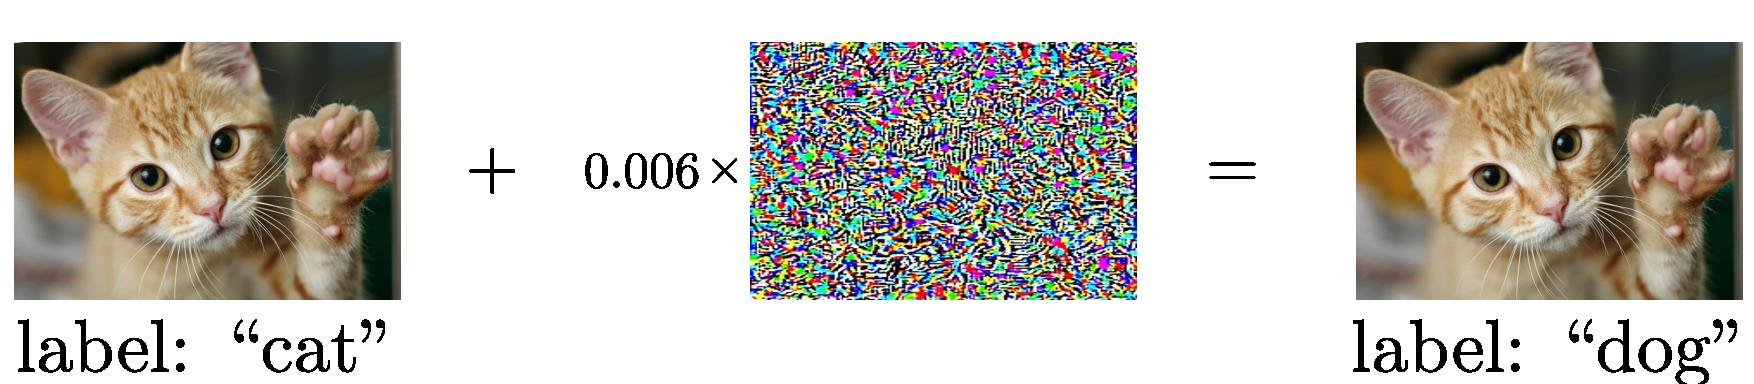
\includegraphics[width=\textwidth]{figures/main/ch1-introduction/ExampleAdversarialCatDog.pdf}
  \caption{Example of Adversarial Attack on an image.}
  \label{figure:ch1-adversarial_image_example}
\end{figure}

Large neural networks due to a high complexity and expressivity exhibit instability to small perturbations of their inputs.
The best example of this phenomenon is the vulnerability of neural networks to \emph{adversarial examples}, \ie, imperceptible variations of natural examples, crafted to deliberately mislead the models~\cite{globerson2006nightmare,biggio2013evasion,szegedy2013intriguing}.
The \Cref{figure:ch1-adversarial_image_example} gives an example of an adversarial attack on an image.
The small perturbation (center) is added to the original image (left) leading to an adversarial image (right).
This behavior can cause serious security problems when neural networks used for critical decision-making (\eg self-driving cars).

% The instability of neural networks to small input perturbations has led them to be vulnerable to \emph{adversarial examples}, \ie, imperceptible variations of the natural examples, crafted to deliberately mislead the models.

The study of security properties of learning algorithms is a research field known as \emph{adversarial machine learning} which dates back to 2004 \cite{dalvi2004adversarial}.
More recently, the work of \citet{szegedy2013intriguing} has brought considerable attention to adversarial examples in the context of Deep Learning.
Since then, a number of work has been published in designing attacks and defenses \cite{szegedy2013intriguing,goodfellow2014explaining,papernot2016limitations,madry2018towards,carlini2017towards,pinot2019theoretical}.
\emph{Adversarial Training} (AT), one of the first effective methods to protect against adversarial examples, was introduced by \citet{goodfellow2014explaining} and later improved by \citet{madry2018towards}.
It consists of augmenting training batches with adversarial examples generated during the training procedure.
More recently, a new method \cite{farnia2018generalizable} based on the regularization of the Lipschitz constant of the network has been proposed which linked the generalization capabilities of neural networks to their Lipschitz constant; therefore, a reduced Lipschitz constant could lead to a better generalization.
Although these methods improve the robustness of neural networks, the accuracy obtained ``under attack'' is far from state-of-the-art and therefore security risks are still present.

In this thesis, we build robust neural networks by studying the properties of the structure of convolution.
We devise a new upper bound on the largest singular value of convolution layers that is both tight and easy to compute.
Our work is based on the result of~\citet{gray2006toeplitz} which states that an upper bound on the singular value of Toeplitz matrices can be computed from the inverse Fourier transform of the characteristic sequence of these matrices.
From our analysis immediately follows an algorithm for bounding the Lipschitz constant of a convolutional layer, and by extension the Lipschitz constant of the whole network.
Finally, we illustrate our approach on adversarial robustness.
Recent work has shown that empirical methods such as adversarial training offer poor generalization~\cite{schmidt2018adversarially}, and can be improved by applying Lipschitz regularization~\cite{farnia2018generalizable}.
To illustrate the benefit of our new method, we train neural networks with Lipschitz regularization and show that it offers a significant improvement over adversarial training alone.





% In this thesis, we study the properties of structured matrices from the Toeplitz family and make contributions to the field of supervised learning with neural networks.
% This thesis is organized in two parts.
% First, we use circulant matrices, which are a particular case of Toeplitz matrices, to devise a new compact architecture replacing Fully Connected Neural Networks.
% More precisely, we study deep diagonal-circulant neural networks, which are deep neural networks in which weight matrices are the product of diagonal and circulant ones.
% Besides making a theoretical analysis of their expressivity, we introduce principled techniques for training these models: we devise an initialization scheme and propose a smart use of nonlinearity functions in order to train deep diagonal circulant networks.
% Furthermore, we show that these networks outperform recently introduced deep networks with other types of structured layers.
% We conduct a thorough experimental study to compare the performance of deep diagonal circulant networks with state-of-the-art models based on structured matrices and with dense models.
% We show that our models achieve better accuracy than other structured approaches while requiring 2x fewer weights than the next best approach.
% Finally, we train compact and accurate deep diagonal circulant networks on a real-world video classification dataset with over 3.8 million training examples.
% In the second part of this thesis, we study the properties of the structure of convolution to devise a new upper bound on the largest singular value of convolution layers that is both tight and easy to compute.
% Our work is based on the result of~\citet{gray2006toeplitz} which states that an upper bound on the singular value of Toeplitz matrices can be computed from the inverse Fourier transform of the characteristic sequence of these matrices.
% From our analysis immediately follows an algorithm for bounding the Lipschitz constant of a convolutional layer, and by extension the Lipschitz constant of the whole network.
% Finally, we illustrate our approach on adversarial robustness.
% Recent work has shown that empirical methods such as adversarial training (AT) offer poor generalization~\cite{schmidt2018adversarially}, and can be improved by applying Lipschitz regularization~\cite{farnia2018generalizable}.
% To illustrate the benefit of our new method, we train neural networks with Lipschitz regularization and show that it offers a significant improvement over adversarial training alone.


%%%%%%%%%%%%%%%%%%%%%%%%%%%%%%%%%%%%%%%%%%%%%%%%%%%%%%%%%%%%%%%%%%%%%%%%%%%%%%%
\section*{Outline of the Thesis}
\label{section:ch1-outline_of_the_thesis}
%%%%%%%%%%%%%%%%%%%%%%%%%%%%%%%%%%%%%%%%%%%%%%%%%%%%%%%%%%%%%%%%%%%%%%%%%%%%%%%

This thesis is organized in six chapters.
First, \Cref{chapter:ch2-background} gives an introduction on the theory of Toeplitz matrices and on supervised learning and neural networks.
This chapter presents the necessary technical tools we will need for presenting the related work and for our contributions.
\Cref{chapter:ch3-related_work} is dedicated to enumerating the state-of-the-art approaches.
The chapter is divided into two parts.
First, we review techniques to build compact neural networks with an important focus on techniques that use structured matrices.
The second part focuses on presenting regularization methods for improving the robustness of neural networks.
\Cref{chapter:ch4-diagonal_circulant_neural_network} and \Cref{chapter:ch5-lipschitz_bound} constitute our main contributions.
\Cref{chapter:ch4-diagonal_circulant_neural_network} presents results on compact neural networks built from diagonal and circulant matrices.
\Cref{chapter:ch5-lipschitz_bound} presents our new regularization scheme to improve the robustness of neural networks based on the properties of doubly-block Toeplitz matrices.
\Cref{chapter:ch6-conclusion} proposed a discussion and some perspectives on the contributions.
Appendix~\ref{appendix:ap2-diagonal_circulant_neural_networks_for_video_classification} constitutes some complements to~\Cref{chapter:ch4-diagonal_circulant_neural_network}.
It provides additional experiments on video classification with compact neural networks.
Appendix~\ref{appendix:ap3-theoretical_evidence_for_adversarial_robustness_through_randomization} and Appendix~\ref{appendix:ap4-advocating_multiple_defense_strategies_against_adversarial_examples} provide further work on the robustness of neural networks done during this Ph.D. thesis.
Finally, Appendix~\ref{appendix:ap6-publications} enumerates the publications made during this Ph.D. thesis.




